\section{การต่อเติมภาพเฉดเทา}

\hspace{1cm} ในการกล่าวถึงขั้นตอนวิธีการต่อเติมภาพ จะเริ่มต้นด้วยการกล่าวทบทวนเกี่ยวกับการต่อเติมภาพเฉดสีเทา (grayscale image) ก่อน ดังนี้

\hspace{1cm} ให้ $\Omega \subset \mathbb{R}^2$ แทนโดเมนภาพ (image domain) $D \subset \mathbb{R}^2$ แทนโดเมนต่อเติม (ดูรูปที่ \ref{figure:sample-domain}) และ $V \subset [0,\infty)$ และให้ $ u: \Omega \rightarrow V,\ z: \Omega \rightarrow V$ แทนภาพที่ได้รับการซ่อมแซมและภาพที่ต้องการซ่อมแซม ตามลำดับ

\hspace{1cm} ในที่นี้ $ \mathbf{x} = (x,y) \in \Omega $ แทนพิกัดทางกายภาพ (physical position) ของภาพ และ $ u(\mathbf{x}) \in V $ แทนระดับความเข้มของภาพ (image intensity) ที่ $ \mathbf{x} $ และ $ \Omega $ มีรูปร่างสี่เหลี่ยม 

\hspace{1cm} นอกจากนี้เราสามารถสมมติได้โดยไม่เสียหลักการสำคัญว่า $ \Omega = [1,n]^2 $ และ $ V = [0,1] $ เมื่อ $n>0$ เป็นจำนวนเต็มบวก ทั้งนี้ เราจะเรียกภาพ $u,z$ ที่นิยามข้างต้นว่าภาพเฉดสีเทา

\begin{figure}[H]
	\centering
	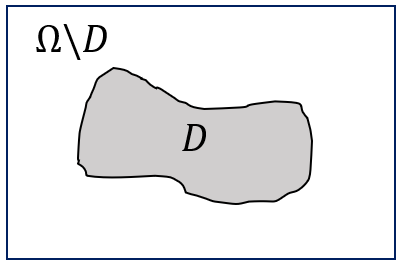
\includegraphics[width=0.375\linewidth]{image/sample-domain.png}
	\caption{$D$ แทนโดเมนต่อเติม}
	\label{figure:sample-domain}
\end{figure}

\subsection{ตัวแบบการต่อเติมภาพเฉดสีเทาที่ใช้การแปรผันรวม}\label{inpaint-model-grayscale}

\hspace{1cm} ในการต่อเติมภาพเฉดสีเทา Chan และ Shen \cite{ref:rof-inpaint-chan-shen} ได้นำเสนอตัวแบบเชิงการแปรผัน (variational model) ที่ใช้เร็กกิวลาร์ไรซ์เซชันแบบการแปรผันรวม (Total variation based regularization) โดยพัฒนาต่อจากตัวแบบ ROF สำหรับการกำจัดสัญญาณรบกวน \cite{ref:ROF-template} ซึ่งตัวแบบเชิงการแปรผันนี้กำหนดโดย
\begin{align}
    \min_{u} \{ \mathcal{J}(u) = \frac{1}{2} \int_{\Omega}\lambda (u-z)^2 d\Omega +  \int_{\Omega}  |\nabla u|  d\Omega \}
\label{e1}
\end{align}

เมื่อ 
\begin{align}
    \lambda=\lambda(\mathbf{x}) = \left \{ \begin{array}{ll}  \lambda_0, & x \in \Omega \setminus D \\ 0, & x \in D  \end{array} \right . 
    \label{e2}
\end{align}
แทนพารามิเตอร์เร็กกิวลาร์ไรซ์เซชัน (regularization parameter) และ $\lambda_0 >0$

\hspace{1cm} โดยแคลคูลัสของการแปรผัน (Calculus of variations) จะได้สมการออยเลอร์ลากรางจ์ที่เกี่ยวข้องกับ (\ref{e1}) เป็น 
\begin{align}
    \left \{ \begin{array}{ll}  - \nabla \cdot  \Big( \dfrac{\nabla u}{|\nabla u|} \Big) + \lambda (u-z) = 0,  & \hspace{1cm} \mathbf{x} \in (1,n)^2 \\ \dfrac{\partial u}{\partial \boldsymbol{n}} = 0, & \hspace{1cm} x \in \partial \Omega \end{array} \right . 
    \label{e3}
\end{align}
เมื่อ $\boldsymbol{n}$ แทนเวกเตอร์หน่วยที่ตั้งฉากกับของของภาพ